\documentclass{tcc}
%%%%%%%%%%%%%%%%%%%%%%%%%%%%%%%%%%%%%%%%%
% Wenneker Article
% Structure Specification File
% Version 1.0 (28/2/17)
%
% This file originates from:
% http://www.LaTeXTemplates.com
%
% Original Authors:
% Frits Wenneker
% Vel (vel@LaTeXTemplates.com)
%
% Adaptation:
% Frankin Coêlho (franklinanthony@eng.ci.ufpb.br)
% Eudisley Anjos (eudisley@ci.ufpb.br)
% Matheus Honório (matheushonorio@eng.ci.ufpb.br)
%
% License:
% CC BY-NC-SA 3.0 (http://creativecommons.org/licenses/by-nc-sa/3.0/)
%
%%%%%%%%%%%%%%%%%%%%%%%%%%%%%%%%%%%%%%%%%

%----------------------------------------------------------------------------------------
%	PACKAGES AND OTHER DOCUMENT CONFIGURATIONS
%----------------------------------------------------------------------------------------

% CI logo colors

\usepackage[brazil]{babel} % English language hyphenation

%\usepackage{authblk}} %Added by Eudis

\usepackage{microtype} % Better typography

\usepackage{amsmath,amsfonts,amsthm,bm} % Math packages for equations

\usepackage[svgnames]{xcolor} % Enabling colors by their 'svgnames'
\definecolor{blueCI}{rgb}{0.0, 0.2, 0.4}
\definecolor{blackCI}{rgb}{0.086, 0.13,0.16}

% \usepackage[hang, small, labelfont=bf, up, textfont=it]{caption} % Custom captions under/above tables and figures

\usepackage{booktabs} % Horizontal rules in tables

\usepackage{lastpage} % Used to determine the number of pages in the document (for "Page X of Total")

\usepackage{graphicx} % Required for adding images

\usepackage{enumitem} % Required for customising lists
\setlist{noitemsep} % Remove spacing between bullet/numbered list elements

\usepackage{sectsty} % Enables custom section titles
\allsectionsfont{\color{blackCI}} % Change the font of all section commands (Helvetica)

\usepackage[colorlinks,linkcolor=blueCI,urlcolor=blueCI,citecolor=blueCI]{hyperref}
\urlstyle{same} % same font as text

\usepackage{lipsum}

%----------------------------------------------------------------------------------------
%	MARGINS AND SPACING
%----------------------------------------------------------------------------------------

\usepackage{geometry} % Required for adjusting page dimensions

\geometry{
	top=1cm, % Top margin
	bottom=1.5cm, % Bottom margin
	left=2cm, % Left margin
	right=2cm, % Right margin
	includehead, % Include space for a header
	includefoot, % Include space for a footer
	%showframe, % Uncomment to show how the type block is set on the page
}

\setlength{\columnsep}{7mm} % Column separation width

%----------------------------------------------------------------------------------------
%	FONTS
%----------------------------------------------------------------------------------------

\usepackage[T1]{fontenc} % Output font encoding for international characters
\usepackage[utf8]{inputenc} % Required for inputting international characters

\usepackage[sfdefault,scaled=.85]{FiraSans}
\usepackage{newtxsf}
%----------------------------------------------------------------------------------------
%	HEADERS AND FOOTERS
%----------------------------------------------------------------------------------------

\usepackage{fancyhdr} % Needed to define custom headers/footers
\pagestyle{fancy} % Enables the custom headers/footers

\renewcommand{\headrulewidth}{0.0pt} % No header rule
\renewcommand{\footrulewidth}{0.4pt} % Thin footer rule

\renewcommand{\sectionmark}[1]{\markboth{#1}{}} % Removes the section number from the header when \leftmark is used

%\nouppercase\leftmark % Add this to one of the lines below if you want a section title in the header/footer

% Headers
\lhead{} % Left header
\chead{\textit{\thetitle}} % Center header - currently printing the article title
\rhead{} % Right header

% Footers
\lfoot{} % Left footer
\cfoot{} % Center footer
\rfoot{\footnotesize \thepage}% de \pageref*{LastPage}} % Right footer, "Page 1 of 2"

\fancypagestyle{firstpage}{ % Page style for the first page with the title
	\fancyhf{}
	\renewcommand{\footrulewidth}{0pt} % Suppress footer rule
}

%----------------------------------------------------------------------------------------
%	TITLE SECTION
%----------------------------------------------------------------------------------------

\newcommand{\authorstyle}[1]{\large\color{blackCI}#1} % Authors style (Helvetica)

\newcommand{\institution}[1]{\footnotesize\usefont{OT1}{phv}{m}{sl}\color{blackCI}#1} % Institutions style (Helvetica)

\usepackage{titling} % Allows custom title configuration

\newcommand{\HorRule}{\color{blueCI}\rule{\linewidth}{1pt}} % Defines the horizontal rule around the title

\newcommand{\TITFONT}{20}

\newcommand{\email}[1]{\normalsize\href{mailto:#1}{#1}\par}

\pretitle{
	\centering \vspace{-30pt} % Move the entire title section up
	\centering \HorRule\vspace{10pt} % Horizontal rule before the title
	\centering \fontsize{\TITFONT}{1.2\TITFONT}\usefont{OT1}{phv}{b}{n}\selectfont % Helvetica
	\centering \color{blackCI} % Text colour for the title and author(s)
}

\posttitle{\par\vskip 15pt} % Whitespace under the title

\preauthor{} % Anything that will appear before \author is printed

\postauthor{ % Anything that will appear after \author is printed
        \centering \vspace{6pt} % Space before the rule
        \vspace{2pt} % Space after the title section
    	\par\HorRule \\ % Horizontal rule after the title
    	\vspace{2pt} % Space after the title section
}

%----------------------------------------------------------------------------------------
%	ABSTRACT
%----------------------------------------------------------------------------------------

\usepackage{lettrine} % Package to accentuate the first letter of the text (lettrine)
\usepackage{fix-cm}	% Fixes the height of the lettrine

\newcommand{\initial}[1]{ % Defines the command and style for the lettrine
	\lettrine[lines=2,findent=4pt,nindent=0pt]{% Lettrine takes up 3 lines, the text to the right of it is indented 4pt and further indenting of lines 2+ is stopped
		\color{blackCI}% Lettrine colour
		{#1}% The letter
	}{}%
}

\usepackage{xstring} % Required for string manipulation

\newcommand{\lettrineabstract}[1]{\color{blackCI}
	\StrLeft{#1}{1}[\firstletter] % Capture the first letter of the abstract for the lettrine
	\initial{\firstletter}\textbf{\StrGobbleLeft{#1}{1}} % Print the abstract with the first letter as a lettrine and the rest in bold
}

%----------------------------------------------------------------------------------------
%	BIBLIOGRAPHY
%----------------------------------------------------------------------------------------

\renewcommand{\refname}{\normalsize{Referências}}

\usepackage[backend=biber,style=ieee,natbib=true]{biblatex} 

\addbibresource{refs.bib} % The filename of the bibliography

\usepackage[autostyle=true]{csquotes} % Required to generate language-dependent quotes in the bibliography

\usepackage{float} % Force the figure to stay where it was determined

\usepackage{nomencl} % List of symbols

\usepackage{listings}
\usepackage{subfig}

\newcommand*{\captionsource}[2]{%
  \caption[{#1}]{%
    #1%
    \\
    \textbf{Fonte:} #2%
  }%
}

\begin{document}
\pagestyle{empty} %retira numeração da página


\begin{figure}[H]
\centering

\includegraphics{latex/imagens/FIAP.png}
\end{figure}

\begin{center}
\Large
Faculdade de Informática e Administração Paulista - FIAP \\
\vspace{3cm}
\begin{figure}[H]
\centering


\includegraphics[width=0.5\textwidth]{latex/imagens/goodwe logo.png}
\end{figure}
\end{center}

% \begin{center}
% \LARGE{\bf \thetitle:}\\
% \Large{\bf \subtitulo}\\
% \end{center}

\vspace{1em}

\begin{center}
\large

\end{center}

\vfill


\begin{center}
\LARGE{RELATÓRIO DE EXPERIÊNCIA DE TRABALHO DA GOODWE}
\end{center}

\vspace{2in}

\begin{center}
\large
São Paulo - SP, \the\year
\end{center}
\afterpage{\addtocounter{page}{1}} %addtocounter incrementa numero da pagina ja que blankpage nao entra no contador%

\newpage

% \begin{center}
%     \rule{3in}{0.4pt} \\ % Linha horizontal
%     % \vspace{0.2cm} % Espaço vertical entre a linha e o texto
%     Texto Abaixo da Linha
% \end{center}

\hfill
\begin{minipage}[t]{0.4\textwidth}
Em atendimento à Lei n. 11.788/2008, apresentamos o relatório das atividades desenvolvidas no estágio curricular supervisionado obrigatório, conforme Termo de Compromisso de Estágio (TCE) e Plano de Atividades de Estágio (PAE) previamente celebrados entre as partes abaixo.
\end{minipage}

\vspace{1.5cm}

\begin{center}    
\begin{minipage}[t]{0.4\textwidth}
    \hrulefill \\
    \centering
    \textbf{Raphael Mischiatti de Souza} \\
    \textit{Rm 563567} \\
    E-mail: r4faelsouza09@gmail.com \\
    % (assinatura)
    \vspace{3cm}
\end{minipage}
\hfill
\\
\begin{minipage}[t]{0.4\textwidth}
    \hrulefill \\
    \centering
    \textbf{Guilherme Martins Rezende} \\
    \textit{Rm 563500} \\
    E-mail: gmrezende07@gmail.com \\
    % (assinatura e carimbo)
    \vspace{3cm}
\end{minipage}


\begin{minipage}[t]{0.4\textwidth}
    \hrulefill \\
    \centering
    \textbf{Nome Completo Sem Abreviação} \\
    \textit{Professor Orientador de Estágio} \\
    E-mail: xxxx@xxxx.xxx \\
    % (assinatura e carimbo)
    \vspace{3cm}
\end{minipage}
\end{center}

\vfill

\begin{center}
    São Paulo \\
    \today
\end{center}

\newpage

\tableofcontents
\newpage

% Uncomment the next line if you want keywords/index terms after the abstract. 
%\textit{\textbf{Keywords}: lorem, ipsum, dolor}
\section{Introdução}

% Bibliography usage
% Whenever you find any source make sure to get the BibTEX citation. Add it to the references.bib file. To cite the reference, use \cite{TitleOfTheReference}
A energia foi um fenômeno natural que nasceu junto a criação do planeta, porém seus estudos começaram tempos depois. Na antiguidade, o filósofo Tales de Mileto foi um dos primeiros a registrar eventos relacionados a energia, mas estudos aprofundados começaram apenas no século XVI. Depois de séculos de estudo, a eletricidade provinda da energia elétrica passou a ser um item indispensável para o século XXI, o que acabou culminando na criação de meios para gerar energia da forma mais econômica possível. Assim, descobriu-se dois grupos de geração, sendo eles as não renováveis, que emitem CO2 para a atmosfera e prejudica a saúde dos seres vivos de forma geral, e as renováveis, que não emitem CO2 sendo mais benéficas para o meio ambiente \cite{MundoEducacao}.
As formas de geração de energia no Brasil e no mundo gira em torno de energias não renováveis, como mostrado na imagem abaixo.

% modificar tamanhos das imagens 
\begin{figure}[H]
    \centering
    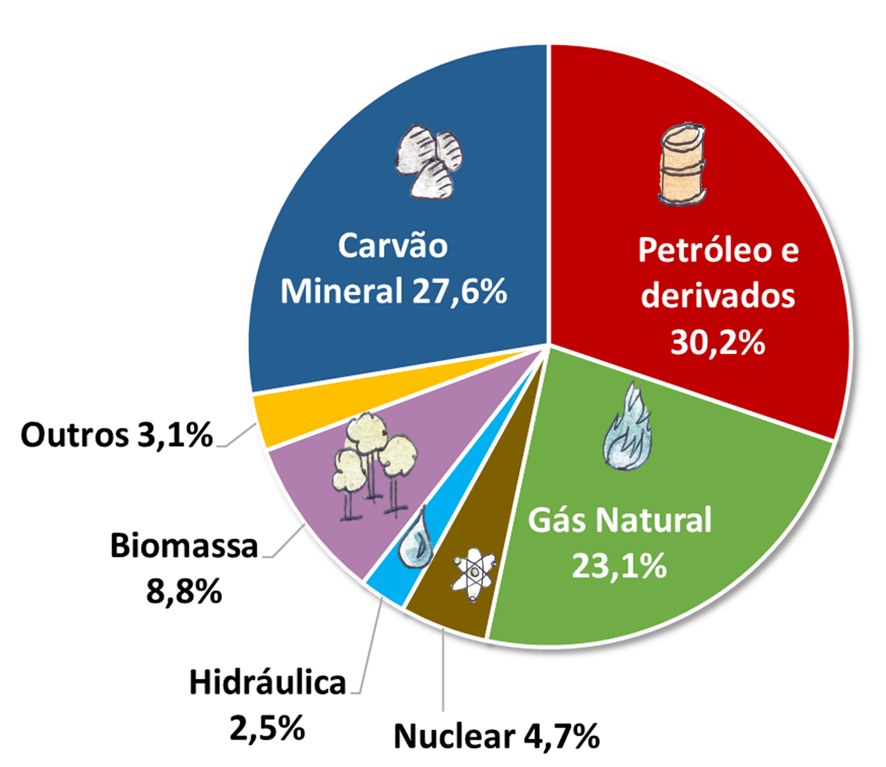
\includegraphics[width=0.4\textwidth]{latex/imagens/energia imagem.png}
    \caption{ https://www.epe.gov.br/pt/abcdenergia/matriz-energetica-e-eletrica}
    \label{fig:bad_images}
\end{figure}

Entretanto, a longo prazo isso torna-se um problema para o ser humano, visto a alta emissão de gás carbônico provindos desses meios de geração o que é prejudicial para a saúde humana. Como em uma matéria do site Agência Brasil, a geração de Co2 deve atingir seu pico em 2025\cite{AgenciaEscola}. Então, uma das formas de reduzir essa emissão seria mudando as fontes de energia para renováveis, como para hidrelétricas, solares etc. Porém, para a energia solar um dos maiores problemas presentes é a dificuldade na manipulação de aparelhos que utilizem esse meio de energia. Além disso, a imprevisibilidade perante as mudanças climáticas pode tornar questão de tempo das pessoas usuárias de energia solar a terem apagões devido a falta de raios UV, o que é prejudicial e afasta as pessoas desse meio de geração \cite{MundoEscola2}.
Logo, a ideia principal do grupo é facilitar e auxiliar os clientes da empresa Goodwe perante a geração de energia, através de um site que mostra gráficos sobre determinadas condições climáticas no dia a dia, momentos do dia para economizar energia e utilização de ia como forma de recomendação do ideal a se fazer e uma ia auxiliar para responder a dúvidas perante a temáticas como clima e geração de energia.


\newpage
% Uncomment the next line if you want keywords/index terms after the abstract. 
%\textit{\textbf{Keywords}: lorem, ipsum, dolor}
\section{Metodologia}
A metodologia do projeto teve como base uma divisão de etapas para a criação do site. Desta forma, foi feita uma vasta pesquisa nos produtos Goodwe tentando identificar pontos de melhora e entendendo como ocorre o funcionamento dos produtos. Assim, com a ideia em mente, o grupo estudou sobre as linguagens JavaScript e Python, além de estudar sobre a linguagem de estruturação HTML e a linguagem de estilização CSS junto ao seu framework Bootstrap. Também utilizamos uma API do tempo para pegar os dados da região que o cliente se encontra.
\newpage
% Uncomment the next line if you want keywords/index terms after the abstract. 
%\textit{\textbf{Keywords}: lorem, ipsum, dolor}
\section{Desenvolvimento}
Como primeiros passos para a implementação do site, foi a criação a base de HTML e uma base de Javascript para testar se a coleta de dados da API estava funcionando. Então era exibido um alert para verificar se era recomendado a pessoa ativar o modo de economia de bateria.


Com o sucesso dessa etapa, deu-se início a estilização com o framework do CSS bootstrap juntamente a um HTML interativo vinculado ao JavaScript para exibir as recomendações na tela perguntando se o usuário gostaria de ativar o modo econômico da bateria, havendo a opção sim e não de resposta. Entretanto, ocorria um erro quando o usuário fazia uma série de comandos que quebravam o código e fazia com que a API não carregasse da forma adequada, mas esse erro foi resolvido rapidamente sem muitos problemas.


Com a parte das recomendações já feita, foi implementado a função de exibição de gráfico com o JavaScript utilizando o site ChartJs para agilizar a criação deles. Assim, foram criados botões para exibir cada um dos gráficos criados e melhorar a interatividade do usuário com a plataforma.


Como último item, foi implementado um agente que recomenda o que o cliente deveria fazer devido as condições daquele dia e um outro que responde a questionamentos relacionados a condições climáticas e geração de energia. A ideia base era utilizar o JavaScript também para o beck-end, focando em apenas uma linguagem de programação para o projeto todo, porém devido a uma série de erros na execução do código o grupo optou por utilizar a linguagem Python para a criação dos agentes.
Para que ocorra a execução do site, no aplicativo VsCode, utiliza o comando python e o nome do arquivo python que carrega a ia que gera as recomendações e a ia auxiliadora para ativá-las.


\newpage

\section{Resultados}
Assim, o projeto se encontra dessa forma até o atual momento:

\begin{figure}[H]
    \centering
    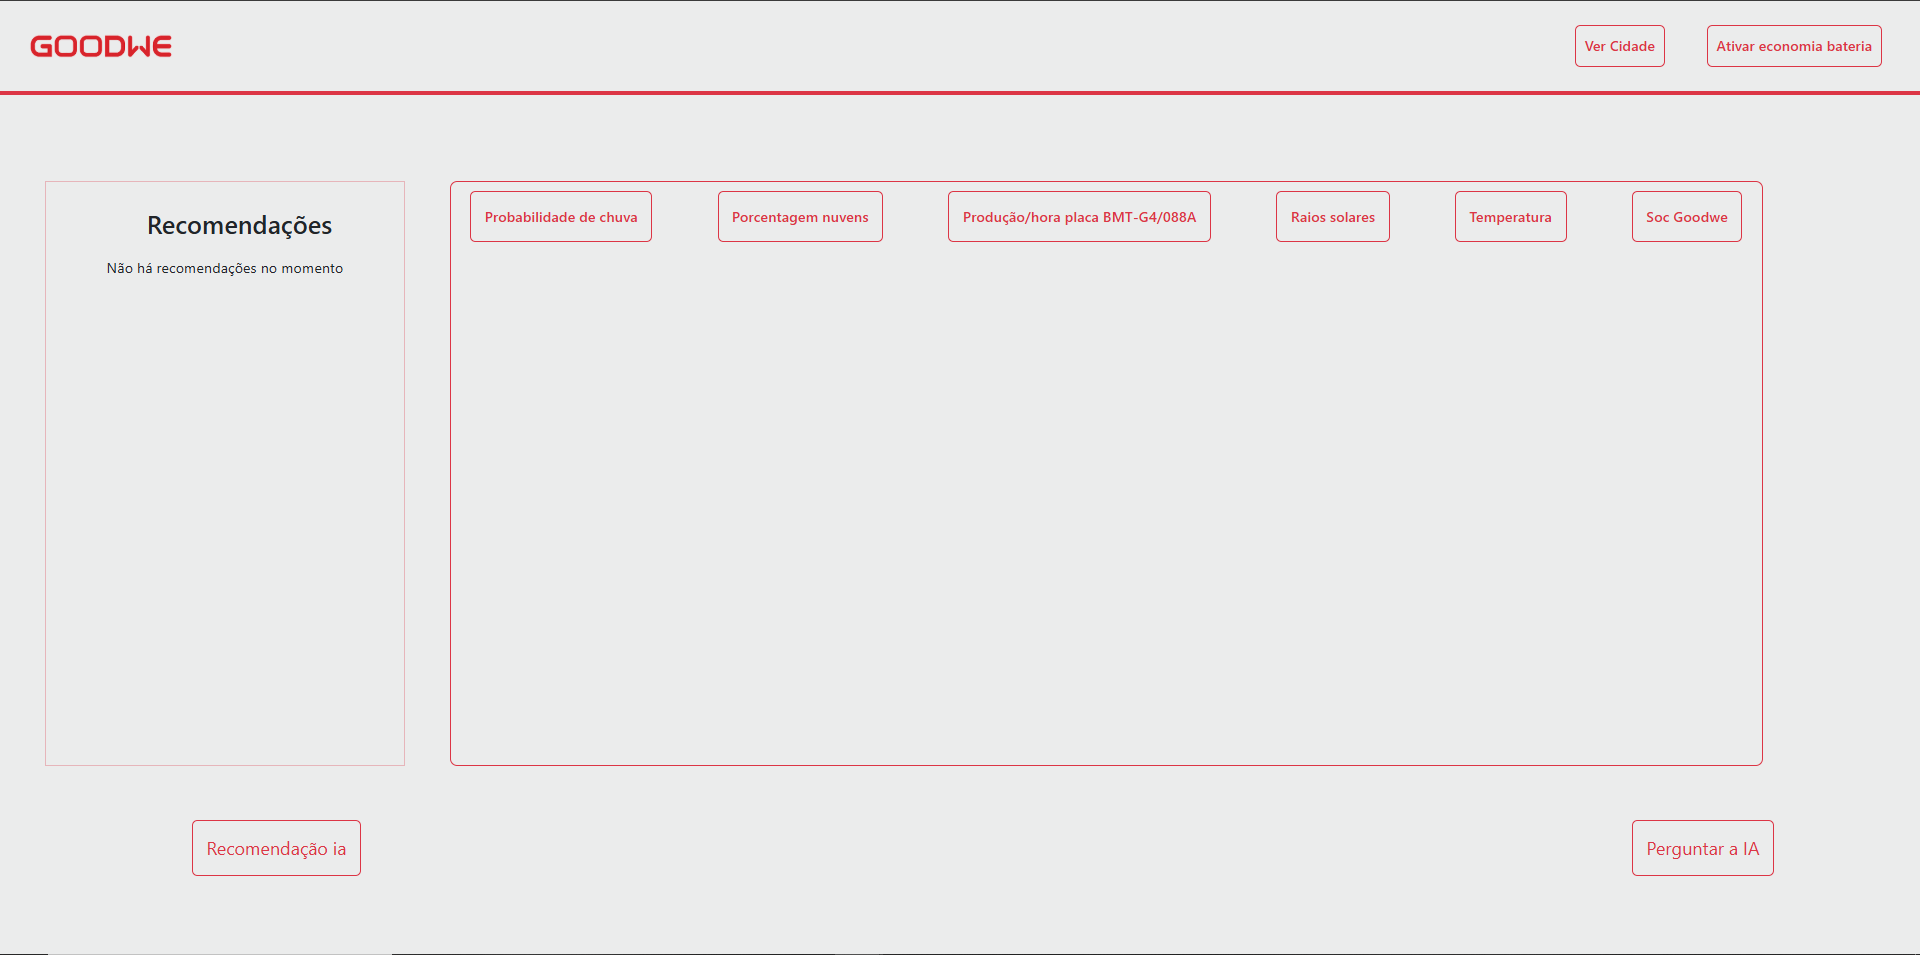
\includegraphics[width=0.9\textwidth]{latex/imagens/imagem site1.png}
    \caption{Referência: autoria própria}
    \label{fig:bad_images}
\end{figure}


\begin{figure}[H]
    \centering
    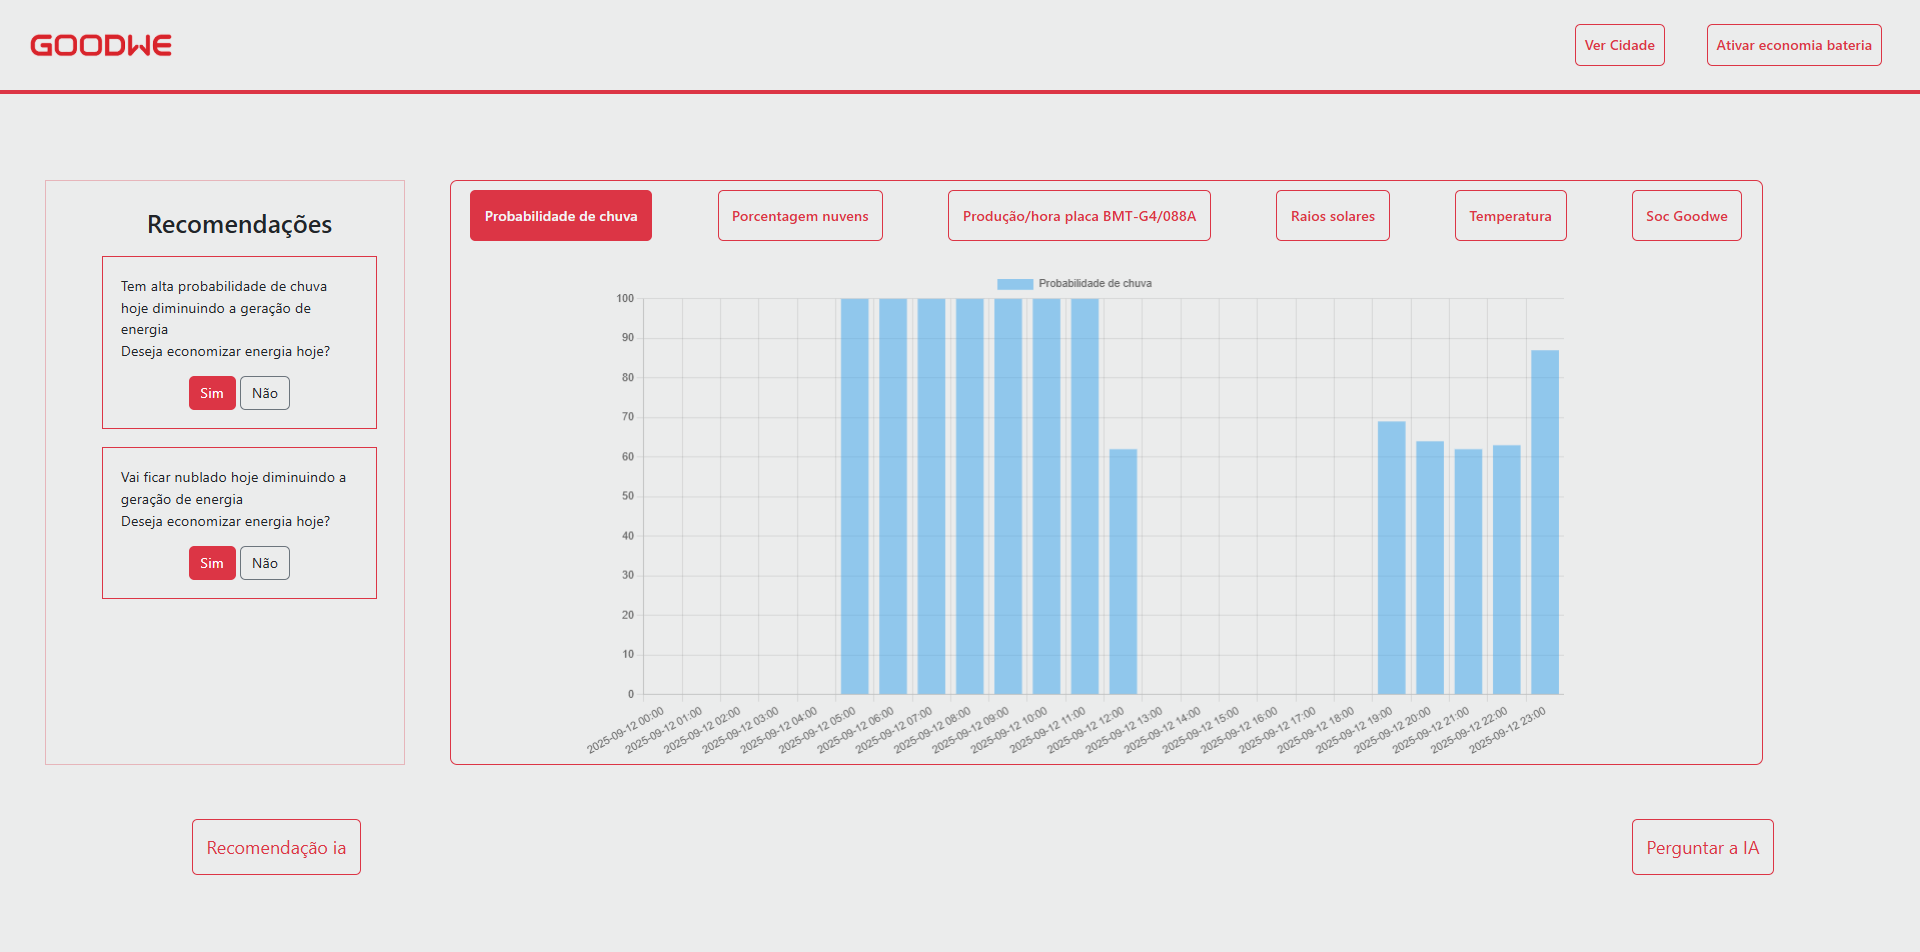
\includegraphics[width=0.9\textwidth]{latex/imagens/imagem site2.png}
    \caption{Referência: autoria própria}
    \label{fig:bad_images}
\end{figure}


Depois do trabalho, ainda falta a parte de conectar o site juntamente com uma assistente virtual e ao inversor da bateria Goodwe para o sistema funcionar. Outro ponto de melhora que é pretendido pelo grupo é um gráfico no último botão exibir informações da bateria do cliente para ter a consciência se precisa de algum ajuste ou como está o seu estado atual.


\newpage

\section{Conclusão}
Depois do trabalho, ainda falta a parte de conectar o site juntamente com uma assistente virtual e ao inversor da bateria Goodwe para o sistema funcionar. Outro ponto de melhora que é pretendido pelo grupo é um gráfico no último botão exibir informações da bateria do cliente para ter a consciência se precisa de algum ajuste ou como está o seu estado atual.


\pagestyle{plain} %mostra numeração da página%
\tableofcontents

\newpage

\printbibliography
\end{document}
